\section{Leave-One-Dataset-Out: Data Volume Does Not Replace Target Labels}
\label{sec:lodo}

If the label count were the bottleneck, pooling every other blade dataset should help. G28 tests this directly. It was pre-registered before any pool was built or any run started.

\subsection{Design}
For each target $T$, two class-agnostic RF-DETR-M arms (640\,px, cosine, seed 0) are scored on $T$'s test set:
\begin{itemize}
\item \textbf{ID-$T$}: trained on $T$'s group training split (WTBD 100 epochs, WTBlade 60).
\item \textbf{X-$T$}: trained for 12 epochs on every other source, twin-free against \emph{all} of $T$. Selection uses a held-out 5\% of X-$T$'s own images~\cite{domainbed}, so $T$ is never seen, not even for selection.
\end{itemize}
Every image of $T$ is an evaluation key for the twin rule: the same file, DINOv2 cosine $\geq0.90$, ORB $\geq25$ inliers, pixel correlation $\geq0.97$ over eight orientations, and the closure of all of these. GAN images and images without boxes are dropped. The rule deliberately sits below the audit's twin thresholds (0.93 and 0.99). Earlier versions of this rule, built for the G27 pool, kept 830 pixel twins and then neighbouring video frames; each failure was logged and fixed before any training. Fig.~\ref{fig:pools} shows the result. X-WTBD has 26{,}065 training images (55{,}845 boxes across its train and held-out images), and X-WTBlade has 14{,}405 (27{,}844). Fig.~\ref{fig:poolaudit} shows the closest pairs an independent audit could find. The highest pixel correlation and cosine to any target image are 0.964/0.827 for X-WTBD and 0.970/0.900 for X-WTBlade.

\begin{figure}[!t]
\centering
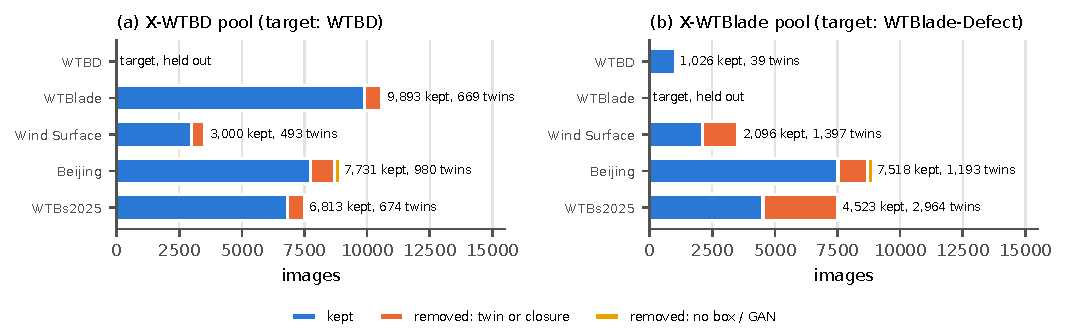
\includegraphics[width=\linewidth]{fig20_pools}
\caption{Composition of the G28 pools: images kept from each source and removed by the twin rule. For X-WTBlade, 2{,}964 WTBs2025 images are removed, since that dataset contains WTBlade-Defect's images.}
\label{fig:pools}
\end{figure}

\begin{figure}[!t]
\centering

\includegraphics[width=0.9\linewidth]{fig21_pool_audit}
\caption{Independent audit of the X-WTBlade pool: the closest remaining pairs by pixel correlation between a kept pool image and a target image. By eye these are similar blades, not copies. The same physical defect from another flight cannot be excluded without capture metadata.}
\label{fig:poolaudit}
\end{figure}

We define the gaps $G_{\mathrm{std}}=\mathrm{ID}-\mathrm{X}$ in standard \apfifty and $G_{\mathrm{reg}}=\mathrm{ID}-\mathrm{X}$ in region AP, and the \emph{convention share}
\begin{equation}
s = 1 - G_{\mathrm{reg}}/G_{\mathrm{std}},
\label{eq:share}
\end{equation}
the part of the gap that is about how boxes are drawn. The direction counted as alive only if, on \emph{both} targets, X reached at least $0.80\times$ ID in region AP and $s\geq0.5$. Both bars were judgment calls fixed before any number existed.

\subsection{Results}
\begin{table}[!t]
\centering
\caption{G28, class-agnostic, test, scene bootstrap (2{,}000 replicates). \emph{Ref} is G27 A0 (class-aware), scored with classes merged; reported, not decisive. \emph{Trivial} is one box over the whole image. Tol.: tolerant \apfifty; Reg.: region AP. \hlnote{} (within each target)}
\label{tab:g28}
\footnotesize
\setlength{\tabcolsep}{2pt}
\begin{tabularx}{\linewidth}{@{}l X r l r r r@{}}
\toprule
Target & Arm & Train & \apfifty & AP$_{50:95}$ & Tol. & Reg. \\
\midrule
WTBD & ID & 745 & \best{72.9} \ci{57.6}{86.3} & \best{41.9} & \best{84.6} & \best{68.9} \\
 & X & 26{,}065 & \textbf{17.7} \ci{11.9}{28.4} & 6.0 & 24.2 & 43.6 \\
 & ref & 745 & \second{66.1} & \second{40.5} & \second{79.7} & \second{65.9} \\
 & trivial & & 0.0 & & & 14.0 \\
\midrule
WTBlade & ID & 2{,}136 & \best{51.7} \ci{48.0}{58.8} & \best{21.5} & \best{65.1} & \best{68.7} \\
 & X & 14{,}405 & \textbf{2.4} \ci{0.8}{3.5} & 0.5 & 3.2 & 37.6 \\
 & ref & 2{,}136 & \second{50.1} & \second{21.3} & \second{61.2} & \second{68.0} \\
 & trivial & & 1.0 & & & 24.2 \\
\bottomrule
\end{tabularx}
\end{table}

\begin{table}[!t]
\centering
\caption{G28 decision. Bars: ratio $\geq0.80$ and share $\geq0.5$ on both targets. ID $-$ X has $P(>0)=1.000$ on every metric of both targets.}
\label{tab:g28-gap}
\scriptsize
\setlength{\tabcolsep}{2pt}
\begin{tabular}{@{}l r r l l l@{}}
\toprule
Target & Ratio & $s$ & $G_{\mathrm{std}}$ [95\% CI] & $G_{\mathrm{reg}}$ [95\% CI] & Verdict \\
\midrule
WTBD & 0.63 & 0.54 & $+55.2$ \ci{+41.7}{+66.4} & $+25.3$ \ci{+14.4}{+33.9} & dead \\
WTBlade & 0.55 & 0.37 & $+49.3$ \ci{+45.0}{+57.2} & $+31.0$ \ci{+26.8}{+34.6} & dead \\
\bottomrule
\end{tabular}
\end{table}

\begin{figure*}[!t]
\centering
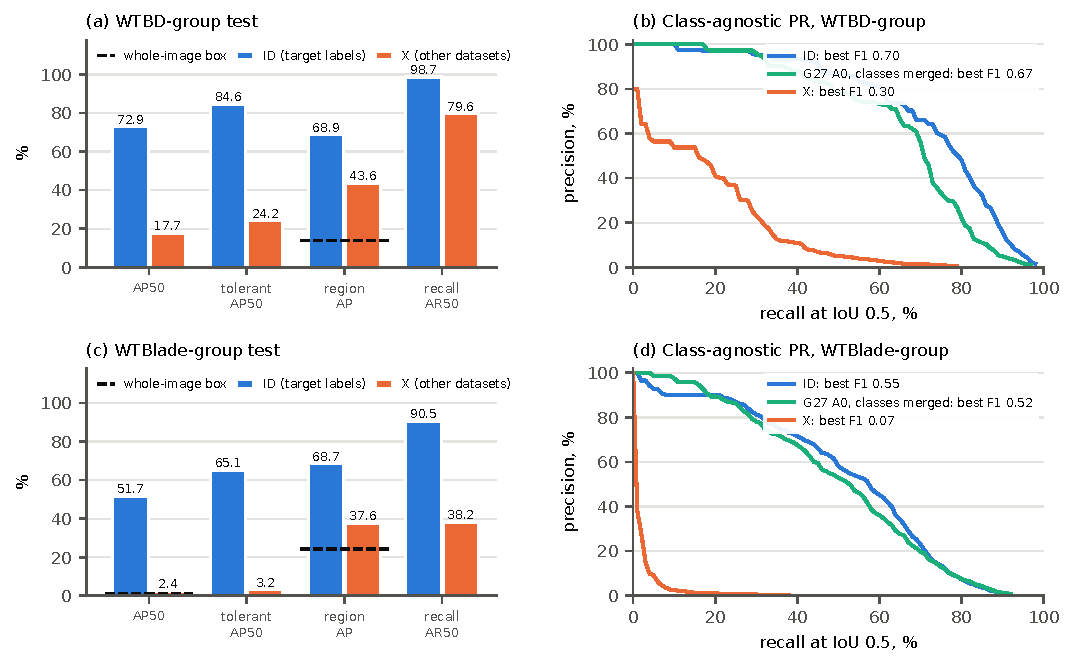
\includegraphics[width=0.96\textwidth]{fig18_g28}
\caption{G28. (a, c) ID and X on target test; dashed lines mark a trivial whole-image detector. (b, d) Class-agnostic precision--recall at IoU 0.5.}
\label{fig:g28}
\end{figure*}

\begin{figure*}[!t]
\centering
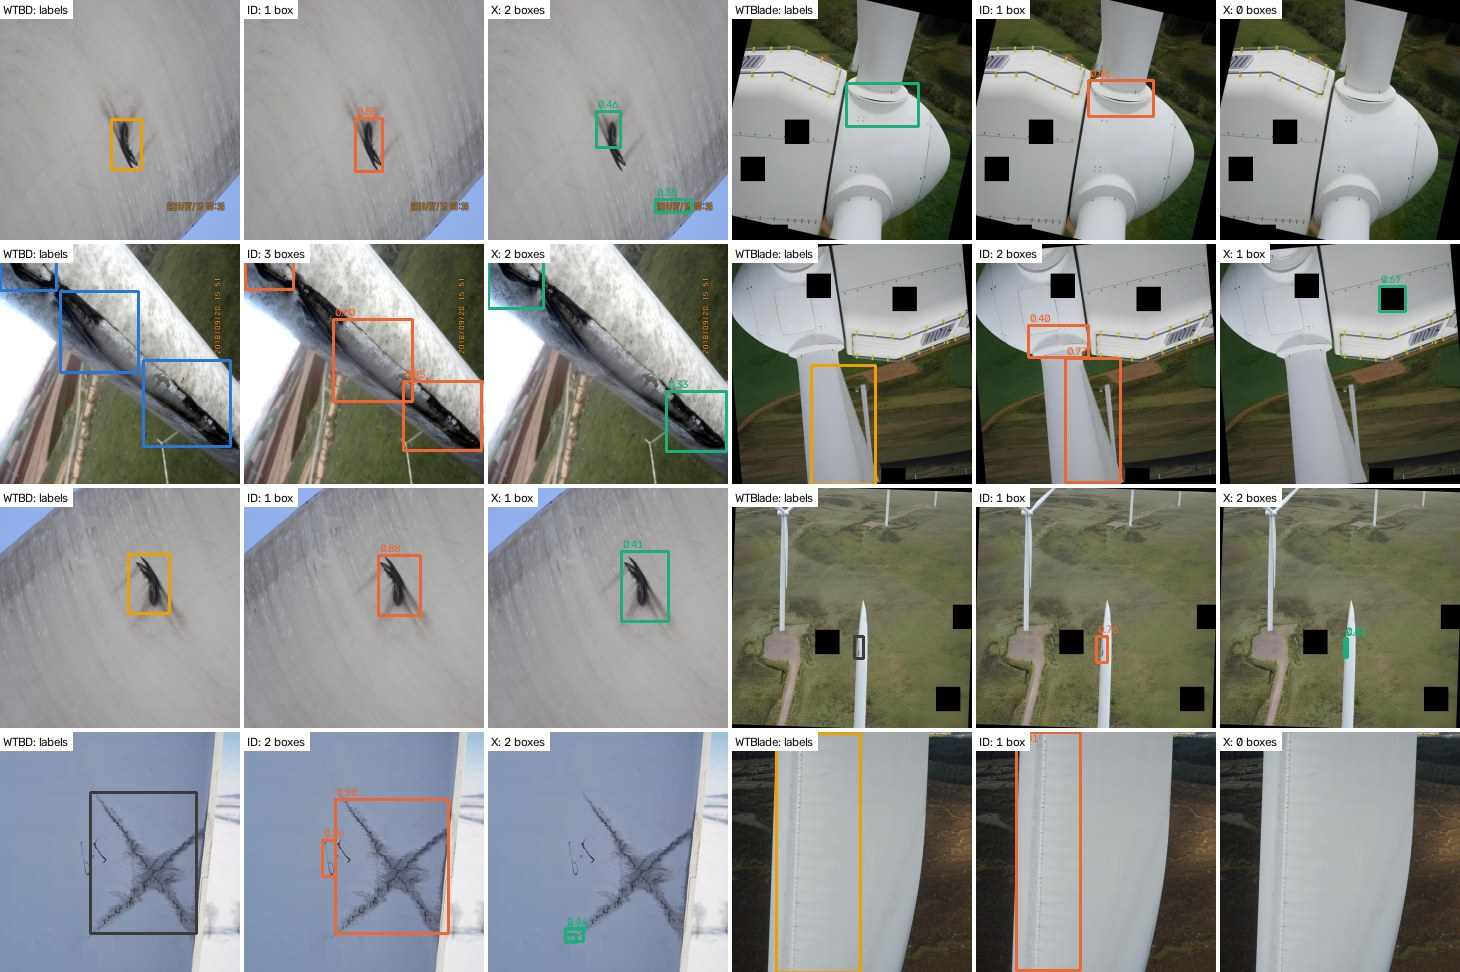
\includegraphics[width=\textwidth]{fig19_predictions}
\caption{Labels, ID and X on random test images (fixed seed), boxes with confidence $\geq$0.3. Left three columns: WTBD-group. Right three: WTBlade-group. X often has the right area or a nearby distractor; it also returns nothing on images where ID is correct.}
\label{fig:predictions}
\end{figure*}

\textbf{The direction fails on both targets} (Tables~\ref{tab:g28}, \ref{tab:g28-gap}; Figs.~\ref{fig:g28}, \ref{fig:predictions}). With 35 times more images from other sources, X still loses to 745 target images by 55 \apfifty points on WTBD-group. The convention explains about half of the gap there and about a third on WTBlade-group; the remainder is a real failure to find the defect. Without the residual pixel-twin images of Fig.~\ref{fig:residual}, the decision is unchanged (ratio 0.64 and 0.56, share 0.55 and 0.39).

\textbf{The model did train.} X-WTBD reached 72.2 \mfifty on its own held-out images at its final epoch. Its region AP is above a trivial detector on both targets (43.6 against 14.0, and 37.6 against 24.2), so it carries information about where defects are. It is not usable as a detector on an unseen dataset, though: X-WTBlade's \apfifty of 2.4 is barely above boxing the whole image (1.0).

\textbf{Why recall and AP disagree on WTBD.} X finds 79.6\% of WTBD labels at IoU 0.5 while scoring 17.7 \apfifty. The reason is that its true boxes rank among many false ones. At recall 10\%, its precision is 54\% against 100\% for ID; at recall 30\% it is 23\% against 95\%. On WTBlade-group, X's precision at recall 10\% is only 3\%, against 90\% for ID. Some false positives are genuine damage of kinds $T$ does not label, so this test is conservative for X.

\textbf{Earlier evidence agrees} (Table~\ref{tab:transfer}). Models trained on one benchmark transfer poorly to the other, and an open-vocabulary foundation detector finds almost nothing without training.

\begin{table}[!t]
\centering
\caption{Generalisation outside one dataset, earlier experiments (BladeYOLO-v2 models; class-agnostic; damage classes only for transfer).}
\label{tab:transfer}
\footnotesize
\begin{tabularx}{\linewidth}{@{}X X@{}}
\toprule
Setting & Result \\
\midrule
WTBlade model on WTBD-group test & \apfifty 5.2 (in-domain 56.3, 58.0); $\Delta$ $-52.5$ \ci{-69.4}{-32.9} \\
WTBD models on WTBlade-group test & \apfifty 4.0, 2.2 (in-domain 47.5); $\Delta$ $-43.9$ \ci{-49.6}{-34.6} \\
Mapped classes across datasets & crack 0.0 both ways; thunderstrike/burn $\leq$7.3 \\
OWLv2~\cite{owlv2}, text queries, no training & \mfifty 3.3 (class-agnostic 5.7); trained on 25\%: 25.0--25.7 \\
OWLv2, few-shot prototypes (25\%) & \mfifty 0.6 (class-agnostic 0.5) \\
\bottomrule
\end{tabularx}
\end{table}
